% NT: Specifically direct students to watch videos and read specific materials; especially the 2nd lecture video.
\section{Introduction to Fourier coefficients}
\label{sec:fouriercoeffintro}

\subsection*{Resources}
\begin{itemize}
    \item Book: 1.4 (\url{https://see.stanford.edu/materials/lsoftaee261/book-fall-07.pdf})
    \item Video: Lecture 2 (\url{https://www.youtube.com/watch?v=1rqJl7Rs6ps})
\end{itemize}

\subsection*{Challenge}
Deduce in a simple way the Fourier coefficients $a_1$ and $b_1$ in the Fourier series
\begin{equation}
    \sum_{k=1}^{N} a_k cos(2 \pi k t) + b_k sin(2 \pi k t)
\end{equation}

for a signal made up of multiple sine signals
\begin{equation}
    \sum_{k=1}^{N} A_k sin(2 \pi k t + \phi_k)
\end{equation}

for the following cases:
\begin{enumerate}
    \item $N=1$, $k=1$, $A_1=1$, $\phi_1=0$
    \item $N=1$, $k=1$, $A_1=1$, $\phi_1=\pi/2$
    \item $N=1$, $k=1$, $A_1=1$, $\phi_1=\pi/5$
\end{enumerate}

Hint: Using $sin(A+B) = sin(A) cos(B) + cos(A) sin(B)$ it should is possible to find the answer without resorting to complex calculation.

\subsection*{Solutions}
\begin{enumerate}
    \item MD5(o\_$a_k$) = a2c1fe\ldots, MD5(p\_$b_k$) = de80c6\ldots
    \item MD5(a\_$a_k$) = 718a6c\ldots, MD5(s\_$b_k$) = f86f0c\ldots
    \item MD5(d\_$a_k$) = 93d647\ldots, MD5(f\_$b_k$) = 9a7b58\ldots
\end{enumerate}

\timebox




%%%%%%%%%%%%%%%%%%%%%%%%%%%%%%%%%
\newpage
%%%%%%%%%%%%%%%%%%%%%%%%%%%%%%%%%

\section{Even and odd functions}
% NT: Need to add practise about even/odd functions occuring as part of fourier functions, maybe in terms of trig cases

\subsection*{Resources}
\begin{itemize}
    \item Wikipedia: \url{https://en.wikipedia.org/wiki/Even_and_odd_functions}
\end{itemize}

\subsection*{Challenge}
Referring in part to the cases in challenge \ref{sec:fouriercoeffintro}, sum the points of all the following TRUE statements:

1 point: Case 1 is an odd function

2 points: Case 1 is an even function

4 points: Case 2 is an odd function

8 points: Case 2 is an even function

16 point: Case 3 is an odd function

32 points: Case 3 is an even function

64 points: $f(x)=Sin(x)$ is an odd function

128 points: $f(x)=Sin(x)$ is an even function

256 points: $f(x)=Cos(x)$ is an odd function

512 points: $f(x)=Cos(x)$ is an even function

1024 points: $f(x)=x$ is an odd function

2048 points: $f(x)=x$ is an even function

\subsection*{Solution}
X

\hash{g}{6a18c0}

\timebox




%%%%%%%%%%%%%%%%%%%%%%%%%%%%%%%%%
\newpage
%%%%%%%%%%%%%%%%%%%%%%%%%%%%%%%%%

\section{Fourier coefficients of sin(x)}
\label{sec:fcsinx}

\subsection*{Resources}
\begin{itemize}
    \item Book: 1.4 (\url{https://see.stanford.edu/materials/lsoftaee261/book-fall-07.pdf})
    \item Video: Lecture 2 (\url{https://www.youtube.com/watch?v=1rqJl7Rs6ps})
\end{itemize}

\subsection*{Comments}
You should be able to follow the derivation of the formula for Fourier coefficients ($C_k$'s) in the video. Feel free to seek help if you have trouble.

\subsection*{Challenge}
1. Write $Sin(x)$ in exponential form.

2. Expand the Fourier series for the function $f(x)$ within the limit $k=-1$ to $k=1$. % NT: Check evaluation by making this a separate question and substituting to check answer.

3. Deduce the Fourier coefficients ($C_k$'s) for the function $Sin(x)$. \emph{This should be possible by inspection, rather than any significant calculation.} % NT: Include C_2, etc too

\subsection*{Solutions}
$C_{-1}$: \hash{h}{28f251}

$C_{0}$: \hash{j}{4fd3f6}

$C_{1}$: \hash{k}{e82a2a}

\timebox




%%%%%%%%%%%%%%%%%%%%%%%%%%%%%%%%%
\newpage
%%%%%%%%%%%%%%%%%%%%%%%%%%%%%%%%%

\section{Fourier Coefficients of 1 + sin(x)}
\label{sec:fcsinxp1}

\subsection*{Resources}
\begin{itemize}
    \item Book: 1.4 (\url{https://see.stanford.edu/materials/lsoftaee261/book-fall-07.pdf})
    \item Video: Lecture 2 (\url{https://www.youtube.com/watch?v=1rqJl7Rs6ps})
\end{itemize}

\subsection*{Comments}
You should be able to follow the derivation of the formula for Fourier coefficients in the video. Feel free to seek help if you have trouble.

\subsection*{Challenge}
Using the same approach as challenge \ref{sec:fcsinx}, deduce for the function $1+sin(x)$ the following Fourier coefficients:

\subsection*{Solutions}
$C_{-1}$: \hash{z}{39e026}

$C_0$: \hash{x}{0ef183}

$C_1$: \hash{c}{89b992}

\timebox




%%%%%%%%%%%%%%%%%%%%%%%%%%%%%%%%%
\newpage
%%%%%%%%%%%%%%%%%%%%%%%%%%%%%%%%%

\section{Relation of positive and negative Fourier coefficients for a real signal}

\subsection*{Resources}
\begin{itemize}
    \item Book: 1.4 (\url{https://see.stanford.edu/materials/lsoftaee261/book-fall-07.pdf})
    \item Video: Lecture 2 (\url{https://www.youtube.com/watch?v=1rqJl7Rs6ps})
\end{itemize}

\subsection*{Challenge}
If the Fourier coefficient $C_1$ is $4 + 6i$, what is the Fourier coefficient $C_{-1}$?

\subsection*{Solution}
X

\hash{m}{36ab38}

\timebox




\stepcounter{section}

%%%%%%%%%%%%%%%%%%%%%%%%%%%%%%%%%
\newpage
%%%%%%%%%%%%%%%%%%%%%%%%%%%%%%%%%

\section{The Fourier series of $f(t)=t$: $C_0$}

\subsection*{Resources}
\begin{itemize}
    \item Book: 1.5, 1.7 (\url{https://see.stanford.edu/materials/lsoftaee261/book-fall-07.pdf})
    \item Video: Lecture 3 (\url{https://www.youtube.com/watch?v=BjBb5IlrNsQ})
\end{itemize}

\subsection*{Challenge}
Considering the function $f(t)=t$ over the interval 0 to 1, calculate the Fourier coefficient $C_0$ using the derived formula for Fourier coefficients. Compare with the average over the interval.

\subsection*{Solution}
X

\hash{aa}{2708ad}

\timebox




%%%%%%%%%%%%%%%%%%%%%%%%%%%%%%%%%
\newpage
%%%%%%%%%%%%%%%%%%%%%%%%%%%%%%%%%

\section{The Fourier series of $f(t)=t$: $C_k$}

\subsection*{Resources}
\begin{itemize}
    \item Book: 1.5, 1.7 (\url{https://see.stanford.edu/materials/lsoftaee261/book-fall-07.pdf})
    \item Video: Lecture 3 (\url{https://www.youtube.com/watch?v=BjBb5IlrNsQ})
\end{itemize}

\subsection*{Challenge}
Considering the function $f(t)=t$, calculate a general expression for the Fourier coefficients $C_k$ where $k \ne 0$.

To check your answer, evaluate the Fourier coefficient for $k=-30$.

\subsection*{Solution}
X

\hash{bb}{8005c7}

\timebox




%%%%%%%%%%%%%%%%%%%%%%%%%%%%%%%%%
\newpage
%%%%%%%%%%%%%%%%%%%%%%%%%%%%%%%%%

\section{The Fourier series of $f(t)=t$ in exponential form}
\label{sec:fstexpform}

\subsection*{Resources}
\begin{itemize}
    \item Book: 1.4 (\url{https://see.stanford.edu/materials/lsoftaee261/book-fall-07.pdf})
    \item Video: Lecture 3 (\url{https://www.youtube.com/watch?v=BjBb5IlrNsQ})
\end{itemize}

\subsection*{Challenge}
1. Write $e^{i 2 \pi k}$ in terms of cosines and sines.

2. Evaluate your expression obtained in (1) for $k=0,1,2,3,4$

3. Write the function $f(t)=t$ evaluated between 0 and 1 in terms of its exponential Fourier series $f(t)=\sum_{k=-N}^{k=N} g(k,t)$ replacing $g(k,t)$ as appropriate.

% NT: Add a challenge with a sum from k=-n to n with n=2
To check your answer, evaluate the Fourier series up to $N=1$ with $t=0.8$.

The graph with increasing values of $N$ looks like this:

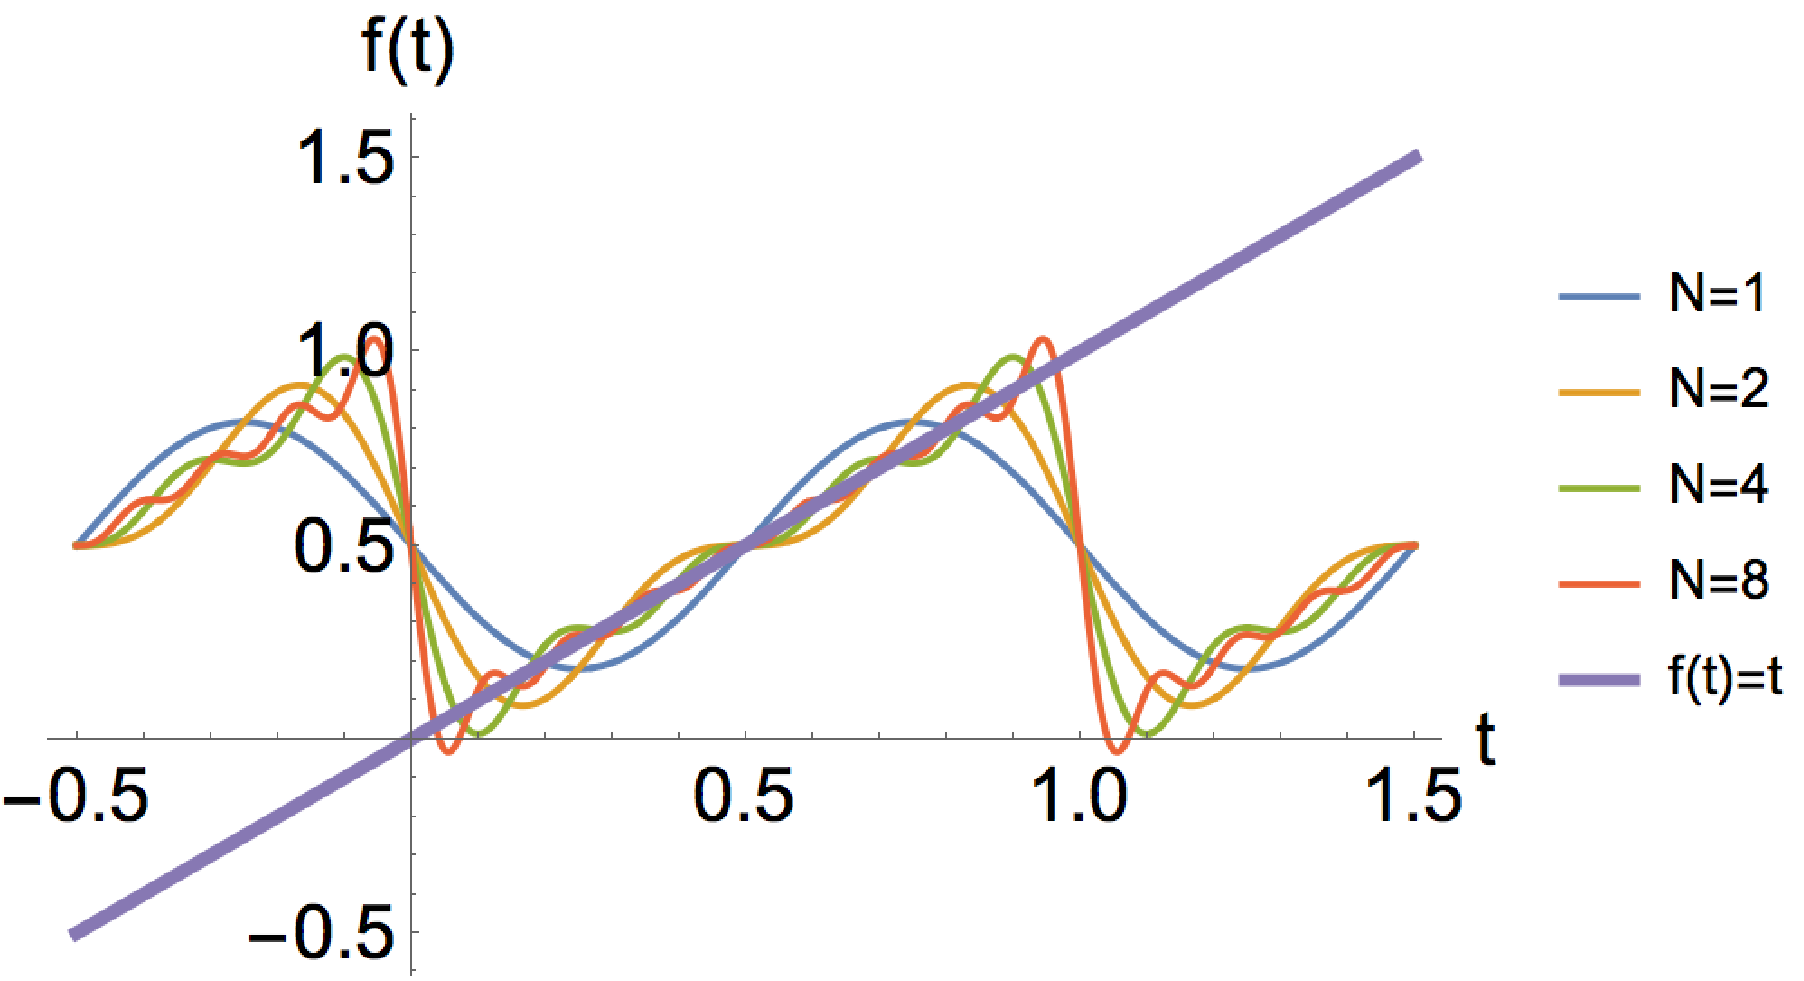
\includegraphics{fourier_series_t.png}

\subsection*{Solution}
X

\hash{cc}{caa033}

\timebox




%%%%%%%%%%%%%%%%%%%%%%%%%%%%%%%%%
\newpage
%%%%%%%%%%%%%%%%%%%%%%%%%%%%%%%%%

\section{The Fourier series of $f(t)=t$ in trigonometric form}
\label{sec:trigexpconvert}

\subsection*{Resources}
\begin{itemize}
    \item Book: 1.5, 1.7 (\url{https://see.stanford.edu/materials/lsoftaee261/book-fall-07.pdf})
    \item Video: Lecture 2 (\url{https://www.youtube.com/watch?v=1rqJl7Rs6ps})
\end{itemize}

\subsection*{Comment}
Since cosine and sine can be written in terms of exponentials, it is possible to switch between Fourier series that are expressed in terms of exponentials and Fourier series that are expressed in terms of sines and cosines. Many textbooks will actually work in terms of these trigonometric forms. Where only sine terms are involved, it is called a ``Fourier sine series'' and where only cosines are involved it's termed a ``Fourier cosine series''. The series have coefficients $a_0$, $a_k$ and $b_k$, in the following fashion:

\begin{equation}
    \label{eq:fsoftintrigform}
    f(t) = \frac{a_0}{2} + \sum_{k=1}^{k=N} a_k cos(2 \pi k t) + b_k sin(2 \pi k t)
\end{equation}

Note that the sum here goes from $k=1$ to $k=N$, in contrast to the exponential form of Fourier series which goes between $k=\pm N$.

\subsection*{Challenge}
1. Write $sin(x)$ in the form of an exponential sum:
\begin{equation}
    sin(x)=\sum_{k=-N}^{k=N} f(k) e^{g(k,x)}
\end{equation}
Your answer in challenge \ref{sec:fcsinx} may help you.

What is $f(k)$, $g(k,x)$ and $N$? To check your answers for $f(k)$ and $g(k,x)$, substitute $k=1$ and $x=2$ as appropriate into your expressions for $f(k)$ and $g(k,x)$.

2. By converting from an exponential-form sum ($\sum_{k=-N}^{k=N}$) to a trigonometric-form sum ($\sum_{k=1}^{k=N}$), re-write the series obtained in challenge \ref{sec:fstexpform} in terms of a trigonometric infinite series (ie, using sines and cosines). To check your answer, evaluate the Fourier series with $N=1$ with $t=0.8$ and ensure that you get the same answer as you did for challenge \ref{sec:fstexpform}.
% NT: Put re-arranging practise into another challenge and make it in more depth (cosines, and both directions). Otherwise students try to use formula instead. Need practise about switching from sums from -infty to sums from 1

3. You should find you are left with an expression only in terms of sine or cosine. Which is it, and how is this related to even/odd functions?

\subsection*{Solution}
\emph{(See the hash examples about entering imaginary numbers)}

$f(k)$: \hash{iiif}{3979fa}

$g(k)$: \hash{iiig}{6cd239}

$N$: \hash{iiin}{e3f634}

\timebox




%%%%%%%%%%%%%%%%%%%%%%%%%%%%%%%%%
\newpage
%%%%%%%%%%%%%%%%%%%%%%%%%%%%%%%%%
\section{Periods other than unity}
\label{sec:nonunitperiods}

\subsection*{Resources}
\begin{itemize}
    \item Book: 1.6.1 (\url{https://see.stanford.edu/materials/lsoftaee261/book-fall-07.pdf})
\end{itemize}

\subsection*{Comment}
Please read the resource. There, $c_n$ is illustrated for an arbitrary period $T$ going from $0$ to $T$, but you do not need to start from $0$. If instead you want to approximate a function from time $T_0$ to $T_0+T$, you can simply swap the integration limits (ie, $T_0$ instead of $0$ and $T_0+T$ for $T$).

\subsection*{Challenge}
\subsubsection*{Part I}
1. By expanding the exponential out in terms of sine and cosine, determine the numerical value of $e^{i \pi k}$ for $k=0,1,2,3,4$.

2. Assuming $k$ can only be an integer, determine the value of $N$ in the formula $e^{i \pi k} = N^k$ and the value of $M$ in the formula $e^{i 2 \pi k} = M^k$.

\subsubsection*{Part II}
Determine $C_0$ and $C_k$ for the following square-wave functions using exponential fourier-series representation:

\vspace{2em}
1.
\begin{equation}
    f(t)=
    \begin{cases}
        1 & \text{for } 0<t<1 \\
        0 & \text{for } 1<t<2
    \end{cases}
\end{equation}

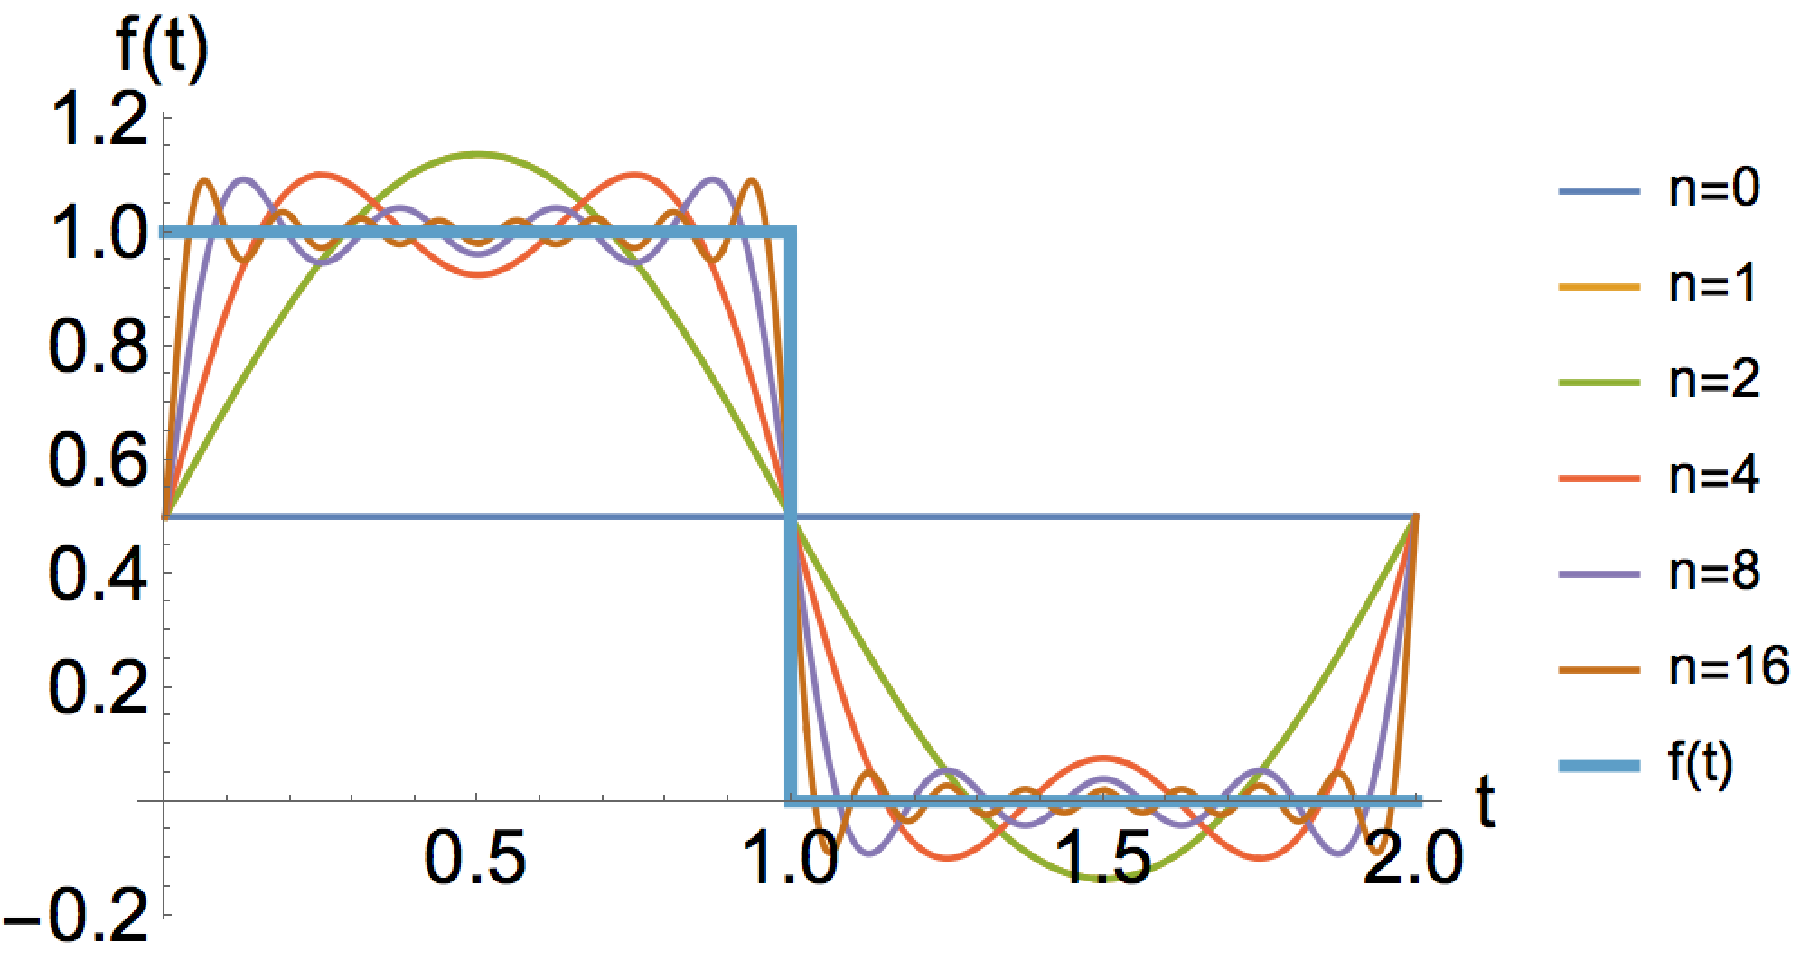
\includegraphics[scale=0.5]{fourier_series_square_wave_01_2.png}

\vspace{2em}
2.
\begin{equation}
    f(t)=
    \begin{cases}
        1 & \text{for } 0<t<\frac{1}{2} \\
        0 & \text{for } \frac{1}{2}<t<1
    \end{cases}
\end{equation}

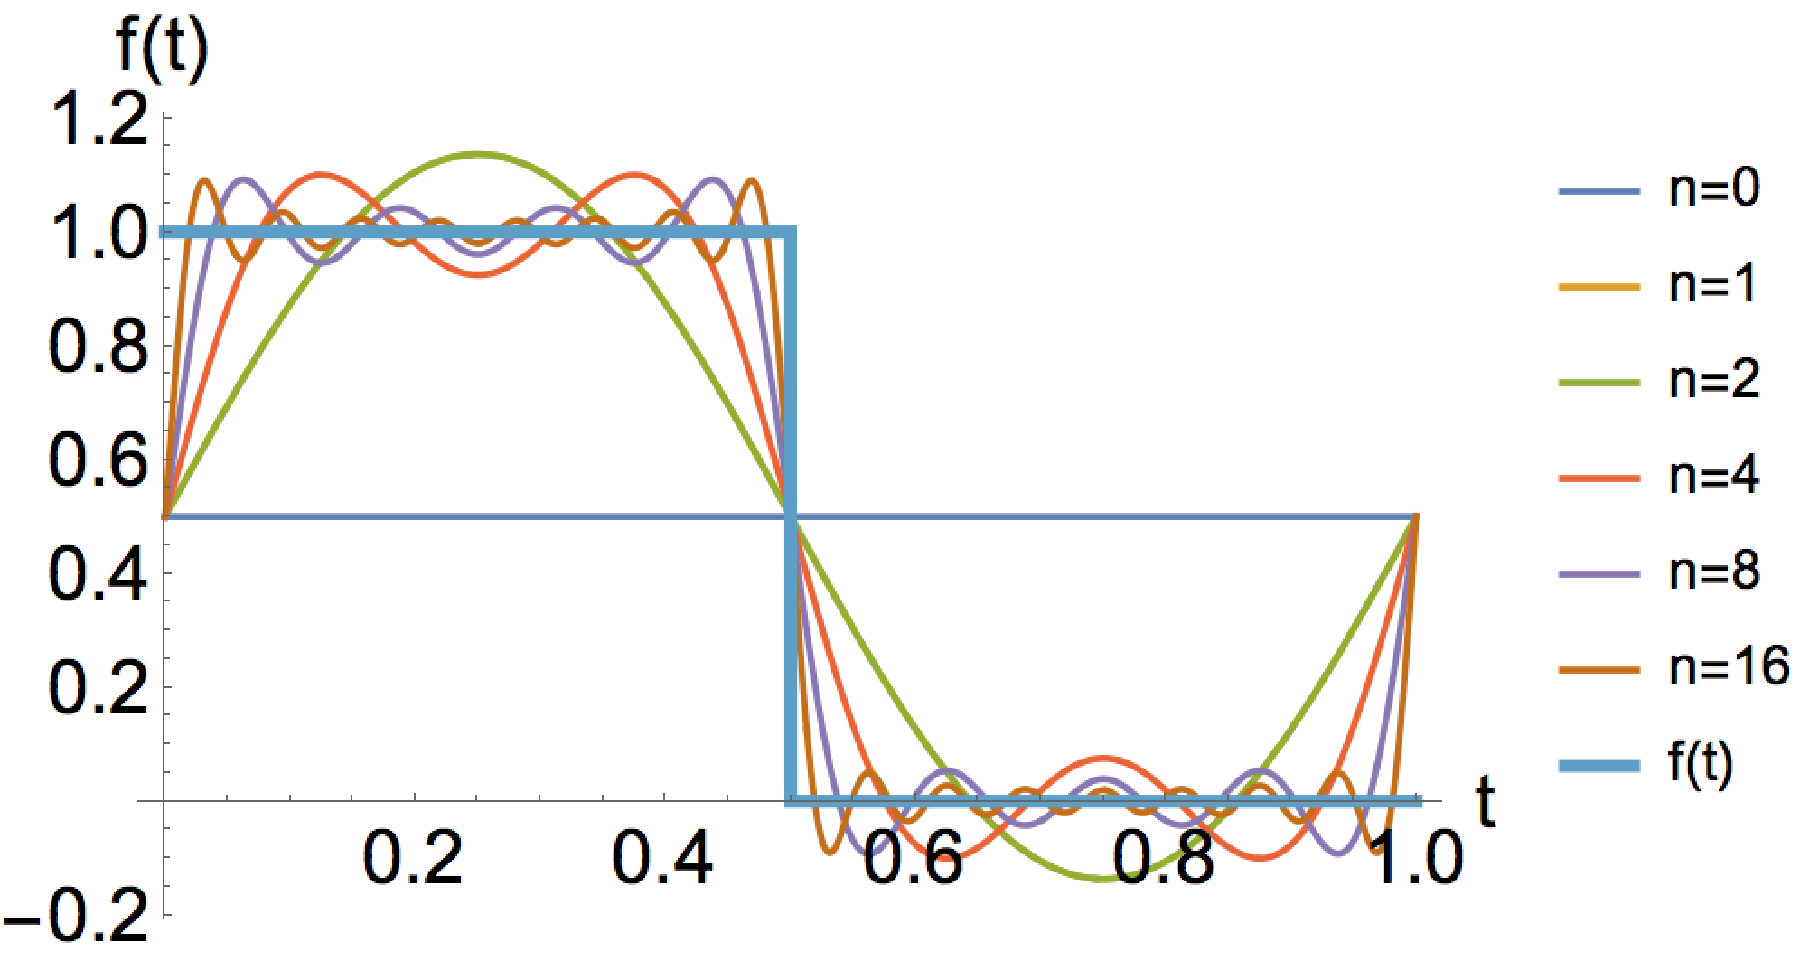
\includegraphics[scale=0.5]{fourier_series_square_wave_00p5_1.png}

\vspace{2em}
3. \emph{(Do not try to simplify the exponentials beyond cosines and sines)}
\begin{equation}
    f(t)=
    \begin{cases}
        1 & \text{for } \frac{1}{8}<t<\frac{7}{8} \\
        0 & \text{for } \frac{7}{8}<t<\frac{9}{8}
    \end{cases}
\end{equation}

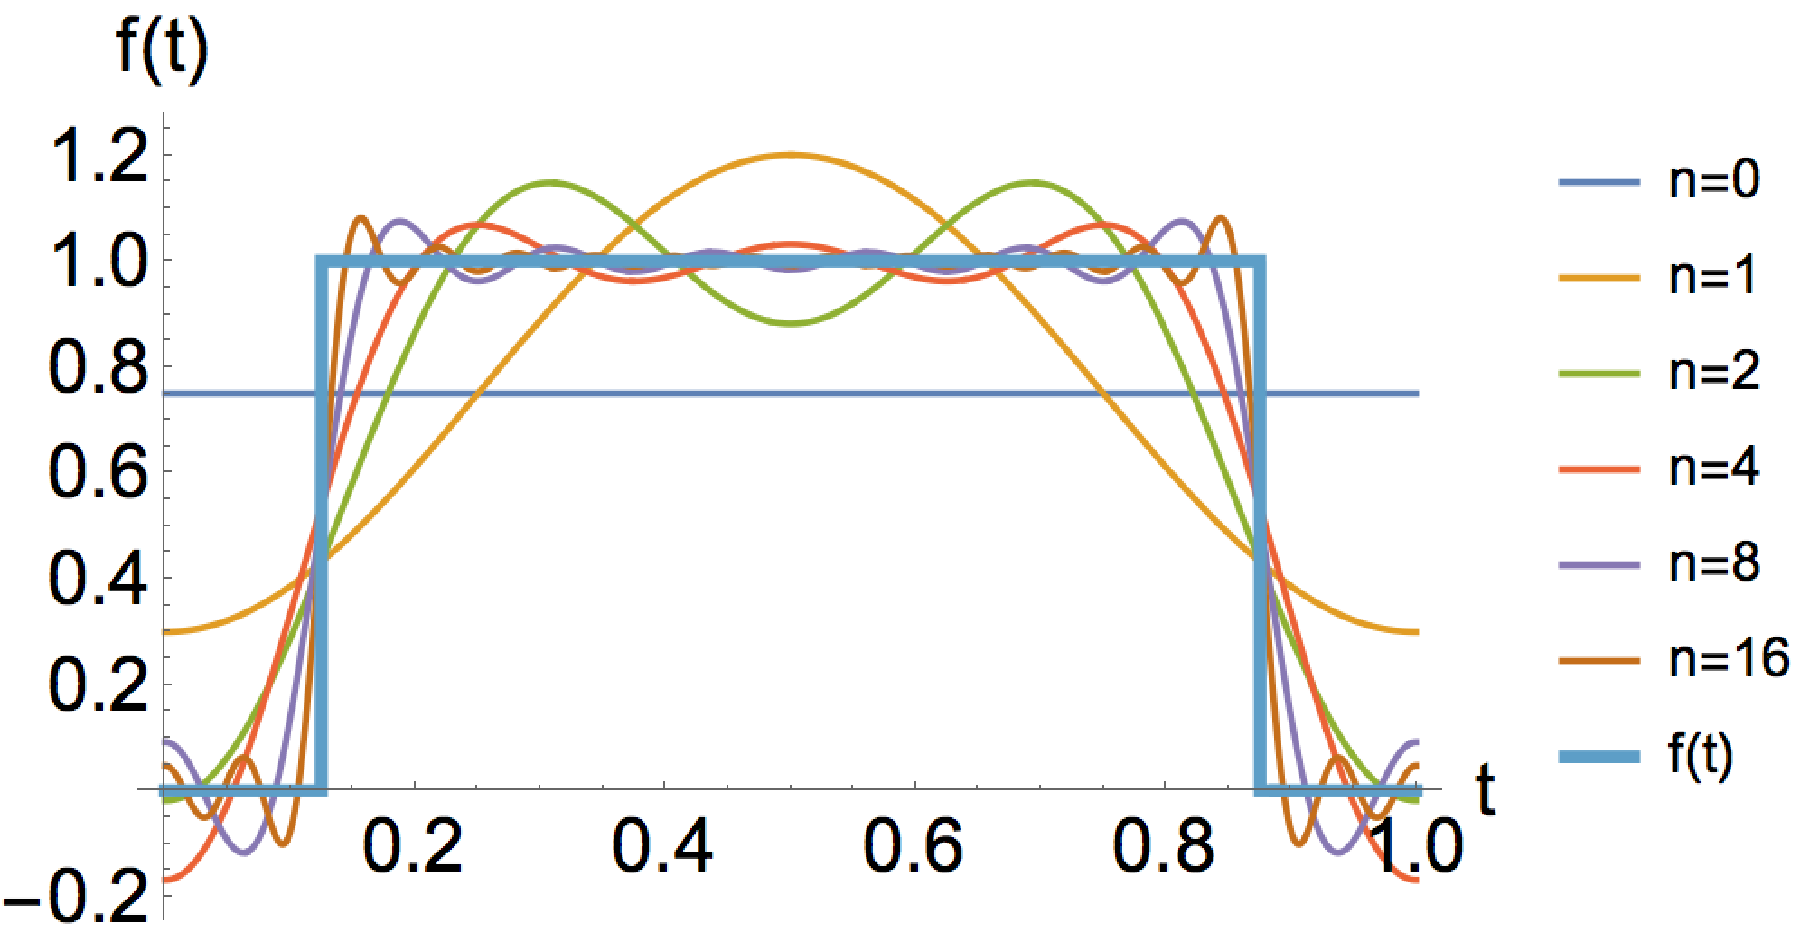
\includegraphics[scale=0.5]{fourier_series_square_wave_eighths.png}

\subsubsection*{Part III}
1. Express each of the square-waves above in terms of an exponential fourier series $f(t)=\sum_{k=-N}^{k=N} g(k,t)$, changing $g(k,t)$ for the exponential fourier series expression. To check your expressions, evaluate the series for $t=1$ with $N=1$.

\subsection*{Solution}
\subsubsection*{Part I}
1.\\
$k=0$: \hash{ddk0}{1b3914}\\
$k=1$: \hash{ddk1}{da2480}\\
$k=2$: \hash{ddk2}{67efb2}\\
$k=3$: \hash{ddk3}{26a591}\\
$k=4$: \hash{ddk4}{f09b1c}

2.\\
N: \hash{ddn}{f3550e}\\
M: \hash{ddm}{e84cb4}

\subsubsection*{Part II}
1.\\
$C_0$: \hash{dd1c0}{aab052}\\
$C_1$: $\displaystyle \frac{-i}{\pi}$

2.\\
$C_0$: \hash{dd2c0}{c34c5d}\\
$C_1$: $\displaystyle \frac{-i}{\pi}$

3.\\
$C_0$: \hash{dd3c0}{ac102c}\\
$C_1$: $\displaystyle \frac{-1}{\sqrt{2}\pi}$

\subsubsection*{Part III}
1. First square-wave: \hash{dd1sum}{35788a}\\
2. Second square-wave: \hash{dd2sum}{75b60f}\\
3. Third square-wave: 0.30 (in decimal form, but it can be written more neatly with fractions and roots)

\timebox




%%%%%%%%%%%%%%%%%%%%%%%%%%%%%%%%%
\newpage
%%%%%%%%%%%%%%%%%%%%%%%%%%%%%%%%%
\section{Infinite series}

\subsection*{Resources}
\begin{itemize}
    \item Book: 1.7 (\url{https://see.stanford.edu/materials/lsoftaee261/book-fall-07.pdf})
\end{itemize}

\subsection*{Comment}
It is important to understand why some series are infinite, while others are not (well, technically all series are infinite since they all involve sums to $n=\infty$, however for some series the Fourier coefficients are all zero above a certain value of $n$). Here

\subsection*{Challenge}
1. In challenge \ref{sec:fcsinx} and \ref{sec:fcsinxp1} you determined the fourier coefficients for $sin(x)$ and $sin(x)+1$. If you write the function in the form
\begin{equation}
    \label{eq:sinxform}
    sin(x)=\sum_{k=-N}^{k=N} C_k e^{i k x}
\end{equation}
what is $N$ here?

\vspace{1em}
2. Expand $e^{i k x}$ in terms of sine and cosine. Which has the higher frequency? $k=1$ or $k=100$?

\vspace{1em}
3. Referring to the resource, do sharp corners in a function lead to higher or lower frequencies?

\vspace{1em}
4. Does non-periodiciy lead to higher or lower frequencies? In challenge \ref{sec:fstexpform} you calculated the Fourier series for $f(t)=t$. If the series is written in a form similar to equation \ref{eq:sinxform}, what would $N$ be in this case?

\vspace{1em}
5. In general, the Fourier series is a sum to $\pm \infty$, however in some cases the coefficients ($C_k$'s) are zero beyond a certain number of terms. Which of the functions below will have Fourier coefficients that are all zero after a certain number of terms? Sum the points of these functions.

1 point: $x$

2 points: $x^2$

4 points: $cos(2 x) + 3 sin(7 x)$

8 points: $e^{2 \pi i x}$

\vspace{1em}
6. Briefly explain the characteristics of functions that lead to infinite Fourier series and finite Fourier series.

\subsection*{Solution}
1. (enter as an integer, without ``.00'') \hash{ee1}{b6cadd} 

2. (``1'' or ``100'') \hash{ee2}{a0bebe}

3. (``lower'' or ``higher'') \hash{ee3}{f0d1f9}

4. \hash{ee4}{7cd9d2}

5. \hash{ee5}{9d1559}

\timebox




%%%%%%%%%%%%%%%%%%%%%%%%%%%%%%%%%
\newpage
%%%%%%%%%%%%%%%%%%%%%%%%%%%%%%%%%
\section{k-symmetry}

\subsection*{Challenge}
Determine what X and Y represent algebraically.
\begin{equation}
    cos(k \pi t) = \frac{1}{2} e^{-k i\pi t} + \frac{1}{2} e^{\bm{X} i \pi x}
\end{equation}
\begin{equation}
    sin(k \pi t) = \frac{1}{2} i e^{\bm{Y} i \pi t} - \frac{1}{2} i e^{k i \pi t}
\end{equation}

To check your answers you may substitute any appropriate values from the following list: $k=2$, $t=1$

\subsection*{Solution}
X

\hash{ff}{942d6f}

Y

MD5(gg\_Y) = a379b8\ldots

\timebox




%%%%%%%%%%%%%%%%%%%%%%%%%%%%%%%%%
\newpage
%%%%%%%%%%%%%%%%%%%%%%%%%%%%%%%%%
\section{Direct trigonometric calculation of a Fourier series: the coefficients}
\label{sec:fs_squarewave}
% NT: Need practise about integration over intervals

\section*{Comment}
This challenge introduces several key concepts at once, including decoupling of integral intervals and periodicity, the concept of a square wave and direct trigonometric evaluation of Fourier series. If you can master this you'll be in a really strong position.

It is hopefully clear now that for real signals, due to the symmetry of the positive and negative k's, one can fully compose Fourier series in terms of sine and cosine. In challenge \ref{sec:trigexpconvert} we saw the formula for the function in terms of Fourier coefficients $a_0$, $a_n$ and $b_n$. While we will not use this approach, it is important to be able to utilise such a formulation since this is the way some books present it and some people have learnt it. Therefore, without proof, the coefficients can be calculated using

\begin{equation}
    a_k = \frac{2}{T} \int_{t_0}^{t_0+T} f(t) Cos(2 \pi k t/T)
\end{equation}
\begin{equation}
    b_k = \frac{2}{T} \int_{t_0}^{t_0+T} f(t) Sin(2 \pi k t/T)
\end{equation}

\subsection*{Challenge}
Using the direct trigonometric Fourier series, obtain a general expression for the $a_k$ and $b_k$ coefficients for the square-wave signal with periodicity 4:

\begin{equation}
    f(t)=
    \begin{cases}
        1 & \text{for } -1<t<1 \\
        0 & \text{for } 1<t<3
    \end{cases}
\end{equation}

Note the symmetry of the problem. Can you see what terms will be zero? To check your solution, calculate $a_k$ and $b_k$ for $k=0$, $k=2$ and $k=3$. Note that you will have to break the integrals into two parts and sum them in order to tackle this problem.

A graph of the function, including the solution for various values of $n$, is shown here:

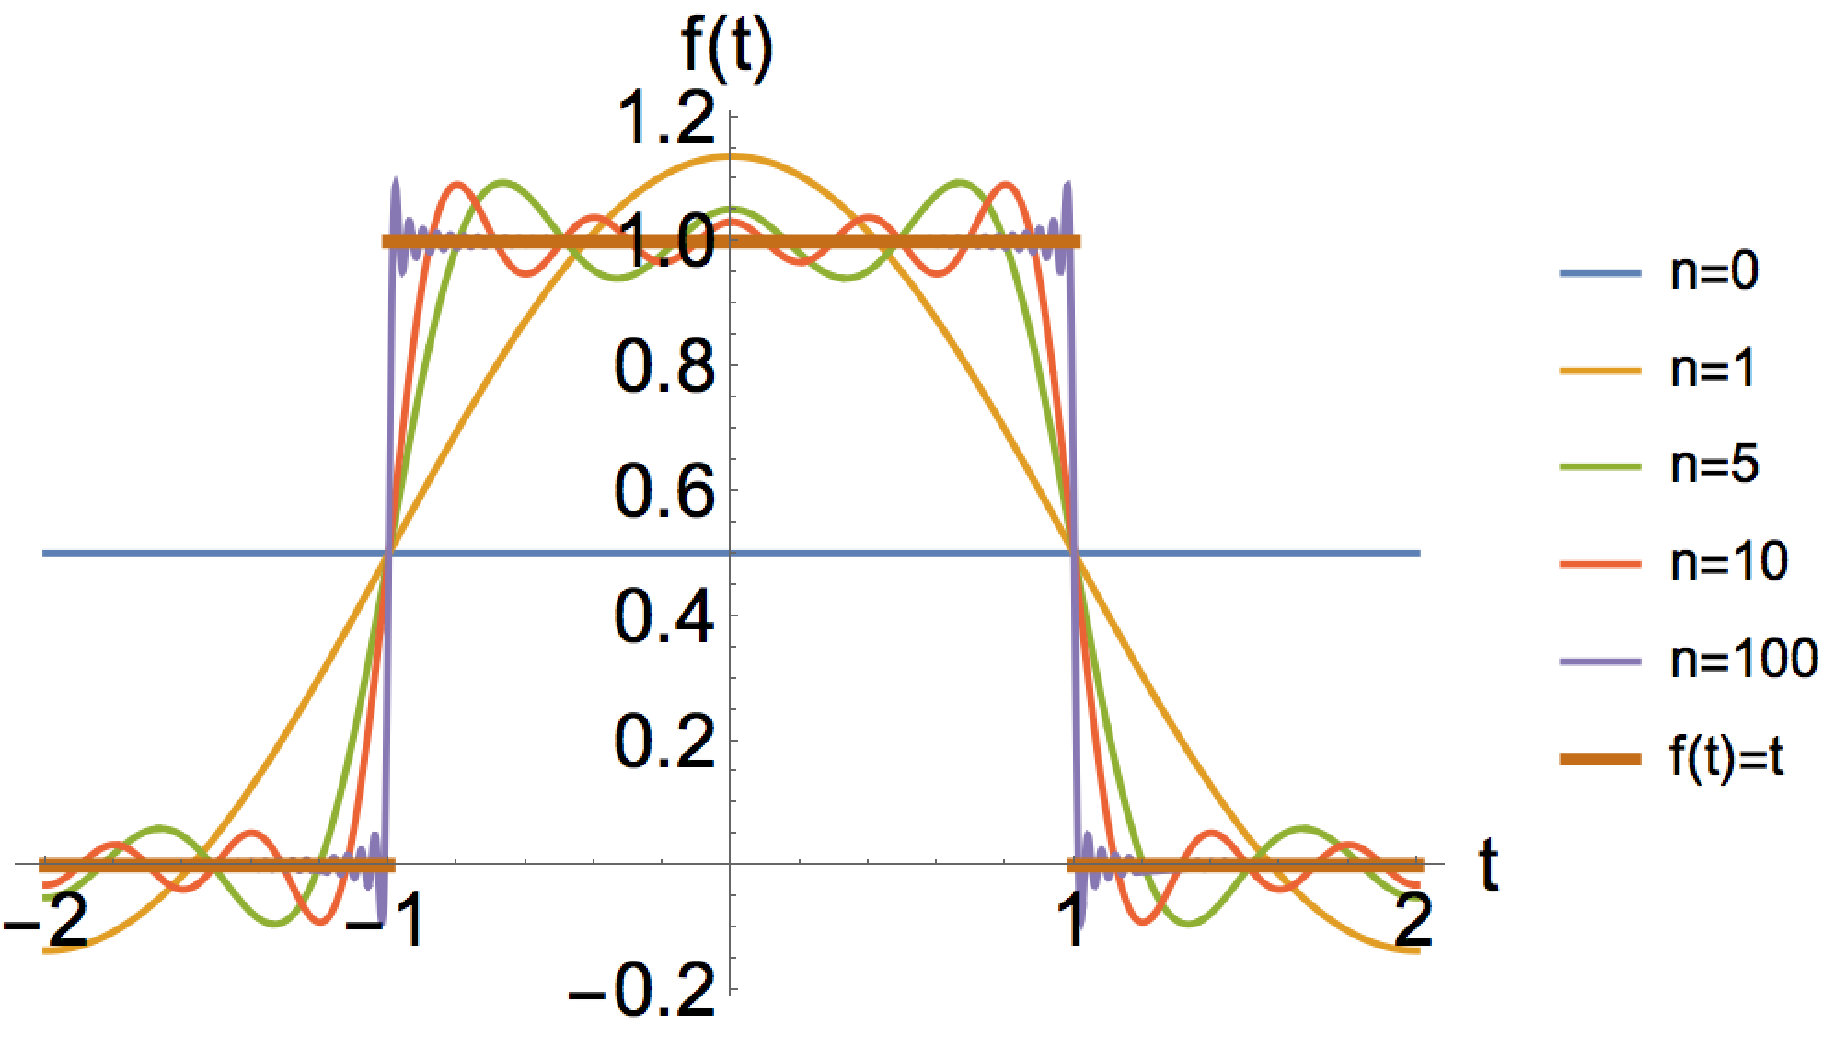
\includegraphics[scale=0.75]{fs_square_wave.png}

\subsection*{Solution}
\begin{tabular}{|l|l|l|}
    \hline
    $k$ & $a_k$ & $b_k$ \\
    \hline
    0 & MD5(hh\_X)=e57c15\ldots & MD5(ii\_X)=377fe2\ldots \\
    2 & MD5(jj\_X)=54aaa1\ldots & MD5(kk\_X)=be063f\ldots \\
    3 & MD5(mm\_X)=b8fce7\ldots & MD5(nn\_X)=b6fbaf\ldots \\
    \hline
\end{tabular}

\timebox




%%%%%%%%%%%%%%%%%%%%%%%%%%%%%%%%%
\newpage
%%%%%%%%%%%%%%%%%%%%%%%%%%%%%%%%%
\section{Direct trigonometric calculation of a Fourier series: the series}

\subsection*{Challenge}
Calculate the Fourier series for the square wave introduced in challenge \ref{sec:fs_squarewave} using direct trigonometric calculation for up to $k=3$ (equation \ref{eq:fsoftintrigform}). Check your solution by evaluating for $t=0.1$.

\subsection*{Solution}
\six{}

\hash{oo}{bd7e5e}

\timebox




%%%%%%%%%%%%%%%%%%%%%%%%%%%%%%%%%
\newpage
%%%%%%%%%%%%%%%%%%%%%%%%%%%%%%%%%
\section{2D orthogonal vectors}

\subsection*{Resources}
\begin{itemize}
    \item Book: 1.9 (\url{https://see.stanford.edu/materials/lsoftaee261/book-fall-07.pdf})
\end{itemize}

\subsection*{Challenge}
Sum the points of the vectors in 2D that are orthogonal:

1 point: (5, 4) and (-1, 1.25)

2 points:  (2, -3) and (-6, 4)

4 points: (-2.25, 1.5) and (2, 3)

8 points: (4.5, 4) and (3, -3.375)

16 points: (6, 4) and (4, -6)

32 points: (5, 1) and (-2, 8.125)

64 points: (0, 1) and (1, 0)

128 points: (1, 1) and (1, 1)

\subsection*{Solution}
\six{}

\hash{pp}{92843f}

\timebox




%%%%%%%%%%%%%%%%%%%%%%%%%%%%%%%%%
\newpage
%%%%%%%%%%%%%%%%%%%%%%%%%%%%%%%%%
\section{Orthonormal basis}

\subsection*{Resources}
\begin{itemize}
    \item Video: \url{https://www.khanacademy.org/math/linear-algebra/alternate-bases/orthonormal-basis/v/linear-algebra-introduction-to-orthonormal-bases}
\end{itemize}

\subsection*{Challenge}
Sum the points of the following vectors that form an orthonormal basis:

1 point :
($\displaystyle \frac{1}{\sqrt{5}}, \frac{2}{\sqrt{5}}$) and
($\displaystyle \frac{2}{\sqrt{5}}, \frac{4}{\sqrt{5}}$)

2 points:
($\displaystyle \frac{2}{\sqrt{5}}$, $\displaystyle \frac{1}{\sqrt{5}}$) and
($\displaystyle \frac{-1}{\sqrt{5}}$, $\displaystyle \frac{2}{\sqrt{5}}$)

4 points:
($\displaystyle \frac{2}{\sqrt{2}}, \sqrt{\frac{7}{8}}, \frac{1}{\sqrt{6}}$),
($\displaystyle -\sqrt{\frac{2}{5}}, \frac{7}{\sqrt{14}}, -\frac{1}{\sqrt{6}}$) and
($\displaystyle \frac{1}{\sqrt{3}},  \frac{1}{5 \sqrt{3}}, -\frac{7}{5 \sqrt{3}}$)

8 points:
($\displaystyle \frac{1}{\sqrt{21}}, \frac{2}{\sqrt{21}}, \frac{4}{\sqrt{21}}$),
($\displaystyle -\sqrt{\frac{2}{7}}, \frac{3}{\sqrt{14}}, -\frac{1}{\sqrt{14}}$) and
($\displaystyle \sqrt{\frac{2}{3}},  \frac{1}{\sqrt{6}}, -\frac{1}{\sqrt{6}}$)

16 points:
($\displaystyle \frac{1}{\sqrt{6}}, \sqrt{\frac{2}{3}}, \frac{1}{\sqrt{6}}$),
($\displaystyle -\frac{1}{\sqrt{2}},  \frac{2 \sqrt{2}}{5}, -\frac{3}{5 \sqrt{2}}$) and
($\displaystyle \frac{1}{\sqrt{3}},  \frac{1}{5 \sqrt{3}}, -\frac{7}{5 \sqrt{3}}$)

32 points:
($0, 2$) and ($2, 0$)

64 points:
($0, 1$) and ($1, 0$)

\subsection*{Solution}
\six{}

\hash{qq}{097fd7}

\timebox




%%%%%%%%%%%%%%%%%%%%%%%%%%%%%%%%%
\newpage
%%%%%%%%%%%%%%%%%%%%%%%%%%%%%%%%%
\section{Natural basis}

\subsection*{Resources}
\begin{itemize}
    \item Book: 1.9 (\url{https://see.stanford.edu/materials/lsoftaee261/book-fall-07.pdf})
\end{itemize}

\subsection*{Challenge}
Sum the components of the following vectors of an orthonormal basis in $\mathbb{R}^{300}$ space:

\begin{itemize}
    \item First component of the first vector
    \item first component of the second vector
    \item 200th component of the 100th vector
    \item 200th component of the 200th vector
    \item last component of the 299th vector
    \item last component of the last vector
\end{itemize}

\subsection*{Solution}
\six{}

\hash{rr}{095c77}

\timebox




%%%%%%%%%%%%%%%%%%%%%%%%%%%%%%%%%
\newpage
%%%%%%%%%%%%%%%%%%%%%%%%%%%%%%%%%
\section{Orthonormal basis for Fourier series}

\subsection*{Resources}
\begin{itemize}
    \item Book: 1.9 (\url{https://see.stanford.edu/materials/lsoftaee261/book-fall-07.pdf})
    \item Video: Lecture 4 (\url{https://www.youtube.com/watch?v=n5lBM7nn2eA})
\end{itemize}

\subsection*{Comment}
The previous challenges have focussed on the orthogonality and orthonormality of vectors. We now make the jump to functions. As chapter 1.9 explains, although its not perfect, the analogy between vectors and functions is a good way to help understand and visualise the role that the terms of a Fourier series play in defining a basis upon which to describe a function.

\subsection*{Challenge}
Starting from the inner product of two terms ($e^{2 \pi i k_1 t}$, $e^{2 \pi i k_2 t}$) of a Fourier series, demonstrate that the terms of a Fourier series form an orthonormal basis. \textbf{Show a full derivation}.

To check your intuition, you may evaluate the following cases:

$X = (e^{2 \pi i k_1 t}, e^{2 \pi i k_1 t})$

$Y = (e^{2 \pi i k_1 t}, e^{2 \pi i k_2 t})$

\subsection*{Solution}
If you are not confident about your derivation, please check with someone else. If there is any step that you do not fully understand, do not hesitate to ask. If you do not understand the connection between previous challenges on vectors and this challenge using functions, do not hesitate to ask someone.

\textbf{X}

\hash{ss}{8f7f41}

\textbf{Y}

MD5(tt\_Y) = 2c669b\ldots

\timebox




%%%%%%%%%%%%%%%%%%%%%%%%%%%%%%%%%
\newpage
%%%%%%%%%%%%%%%%%%%%%%%%%%%%%%%%%
\section{Circles and Fourier series}

\subsection*{Resources}
\begin{itemize}
    \item Video 1: \url{https://www.youtube.com/watch?v=Y9pYHDSxc7g}
    \item Video 2: \url{https://www.youtube.com/watch?v=LznjC4Lo7lE}
\end{itemize}

\subsection*{Comment}
In the first lecture we saw how it was possible to approximate any function given enough circles. Here we link what you have learned back to that first lecture. I strongly recommend viewing the fun and informative videos listed here under Resources. In summary, by building a Fourier series you are representing a function using an orthonormal basis, where each component of the basis can be considered visually as a circle operating with individual radius and frequency on the real-imaginary plane. If, after completing this challenge, that last sentence makes sense to you, then you have achieved the first major goal of this course.

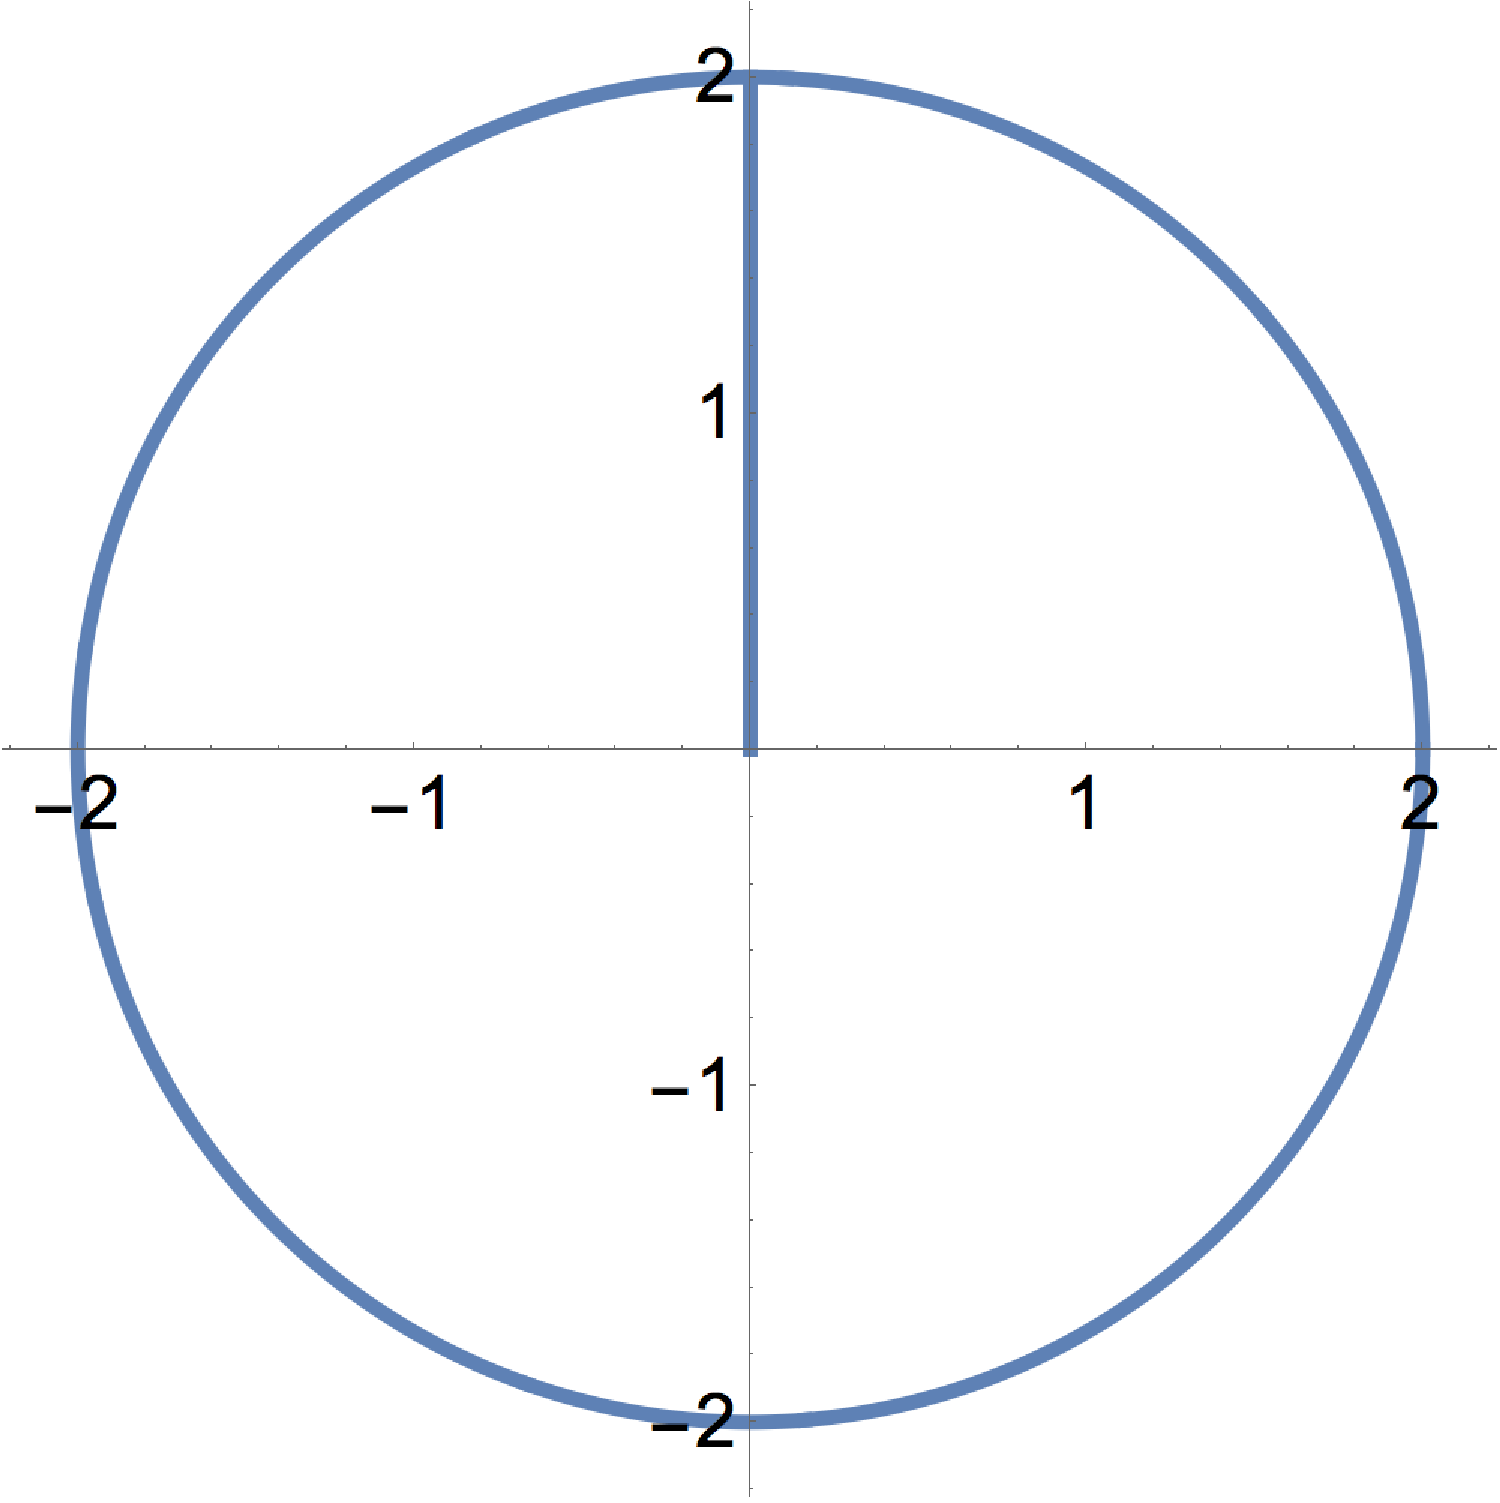
\includegraphics[scale=0.5]{circle.png}

\subsection*{Challenge}
Treating the x-axis as the real axis and the y-axis as the imaginary axis, arrange the equations below in the following order:

\begin{enumerate}
    \item A point moving round on a circle with radius 2 units and frequency 2 Hz
    \item A point moving round on a circle with radius 3 units and frequency 1 Hz
    \item A point moving round on a circle with radius 2 units and a period of 1 second
    \item A point moving round on a circle with radius 3 units and a period of 2 seconds
\end{enumerate}

Equations:

$\displaystyle A e^{2 \pi i k t}$ where $t$ is time in seconds and the values of $A$ and $k$ are as follows:

A: $A=2$, $k=2$ 

B: $A=3$, $k=1$

C: $A=3$, $k=0.5$

D: $A=2$, $k=1$

\subsection*{Solution}
\six{}

\hash{uu}{cb7845}

\timebox




%%%%%%%%%%%%%%%%%%%%%%%%%%%%%%%%%
\newpage
%%%%%%%%%%%%%%%%%%%%%%%%%%%%%%%%%
\section{Gibb's phenomenon}

\subsection*{Resources}
\begin{itemize}
    \item Wikipedia: \url{https://en.wikipedia.org/wiki/Gibbs_phenomenon}
    \item Book: 1.18 (\url{https://see.stanford.edu/materials/lsoftaee261/book-fall-07.pdf})
\end{itemize}

\subsection*{Challenge}
Write a few sentences summarising your understanding of what Gibb's phenomenon is. By what percentage does overshoot of a discontinuity occur given an infinite number of terms?

\subsection*{Solution}
\six{\%}

\hash{vv}{aa19f2}

\timebox



%%%%%%%%%%%%%%%%%%%%%%%%%%%%%%%%%
\newpage
%%%%%%%%%%%%%%%%%%%%%%%%%%%%%%%%%
\section{Partial derivatives}

\subsection*{Challenge}
Determine $u_t$ and $u_{xx}$ for the equation

\begin{equation}
    u(x,t) = 5tx^2 + 3t - x
\end{equation}

To check your answer, substitute $x=3$ and $t=2$ into your answers, as appropriate.

\subsection*{Solution}
$u_t$:\\
\solint{t}{4fb068}

$u_{xx}$:\\
\solint{x}{53502b}




%%%%%%%%%%%%%%%%%%%%%%%%%%%%%%%%%
\newpage
%%%%%%%%%%%%%%%%%%%%%%%%%%%%%%%%%
\section{Heat equation: Periodicity}

\subsection*{Resources}
\begin{itemize}
    \item Book: Section 1.13.1 (\url{https://see.stanford.edu/materials/lsoftaee261/book-fall-07.pdf})
    \item Lecture 4 from 37:00 onwards: (\url{https://www.youtube.com/watch?v=n5lBM7nn2eA}), continuing at the start of lecture 5 (\url{https://www.youtube.com/watch?v=X5qRpgfQld4})
\end{itemize}

\subsection*{Comment}
Here we can learn about an application of Fourier series to solve partial differential equations. This problem was one of the motivations for Fourier to develop the idea of Fourier series.

The motivation for the equation $u_t = \frac{1}{2} u_{xx}$ described in the notes is complicated somewhat by the interpretation in terms of equivalences between electrical and thermal capacitance. If this is not so clear then don't worry about it. At a minimum you should understand the following:
\begin{itemize}
    \item Heat flow is proportional to the gradient of the temperature.
    \item Heat accumulates within a unit volume when the rate of heat flow into that volume is greater than the rate of heat flow out of that volume.
\end{itemize}

\subsection*{Challenge}
The following statements concern a heated ring with circumference 1 and temperature distribution described by $u(x,t)$. Add the points of the statements that are defined by the system to be true:

1 point: $\displaystyle u(x,t) = u(x,t)$

2 points: $\displaystyle u(x,t) = u(x,t+1)$

4 points: $\displaystyle u(x,t) = u(x,t+2)$

8 points: $\displaystyle u(x,t) = u(x+1,t)$

16 points: $\displaystyle u(x,t) = u(x+1,t+1)$

32 points: $\displaystyle u(x,t) = u(x+1,t+2)$

64 points: $\displaystyle u(x,t) = u(x+2,t)$

128 points: $\displaystyle u(x,t) = u(x+2,t+1)$

256 points: $\displaystyle u(x,t) = u(x+2,t+2)$

512 points: The temperature distribution is periodic in space but not time

1024 points: The temperature distribution is periodic in time but not space

2048 points: The temperature distribution is periodic in both space and time

4096 points: The temperature distribution is periodic neither in space nor time


\subsection*{Solution}
\solint{y}{2259d1}




%%%%%%%%%%%%%%%%%%%%%%%%%%%%%%%%%
\newpage
%%%%%%%%%%%%%%%%%%%%%%%%%%%%%%%%%
\section{Heat equation on a ring: derivation}
\label{sec:heateqnfc}

\subsection*{Resources}
\begin{itemize}
    \item Video: \url{https://www.youtube.com/watch?v=yAOCibHPgLA}
    \item Book: Section 1.13.1 (\url{https://see.stanford.edu/materials/lsoftaee261/book-fall-07.pdf})
    \item Lecture 4 from 37:00 onwards: (\url{https://www.youtube.com/watch?v=n5lBM7nn2eA}), continuing at the start of lecture 5 (\url{https://www.youtube.com/watch?v=X5qRpgfQld4})
\end{itemize}

\subsection*{Challenge}
Starting from the heat (diffusion) equation $u_t = u_{xx}/2$, show that the general solution to the heat equation on a ring is given by
\begin{equation}
    u(x,t) = \sum_{n=-\infty}^{n=\infty} c_n(0) e^{-2 \pi^2 n^2 t} e^{i 2 \pi n x}
\end{equation}
and write an expression for $c_n(0)$ in terms of the initial temperature distribution $u(x,0)$.

\subsection*{Solution}
Please compare with your peers during discussion time and ask if there is anything you do not understand.




%%%%%%%%%%%%%%%%%%%%%%%%%%%%%%%%%
\newpage
%%%%%%%%%%%%%%%%%%%%%%%%%%%%%%%%%
\section{Heat equation on a ring: calculation}
\label{sec:heateqn}

\subsection*{Comment}
Remember that any integer multiple of $2 \pi$ in the complex exponential (eg, $e^{i 4 \pi}$ or $e^{i 2 \pi n}$ where $n$ is an integer) is equivalent to having $2 \pi$ in the exponential due to the periodic nature of complex exponentials (ie, that $e^{i 2 \pi} = \cos(2 \pi) + i \sin(2 \pi)$ and $\cos(2 \pi) = \cos(4 \pi) = \cos(6 \pi)$ etc).

\subsection*{Challenge}
Consider an initial heat distribution around a ring. Relative to ambient temperature, the initial temperature distribution follows a cosine distribution with the peak temperature at $x=0$.

1. Write an expression for the initial relative temperature distribution, $u(x,0)$, assuming the ring has a circumference of 1 unit.

2. Determine $c_{n=\pm 1}(0)$ and $c_{n \ne 1}(0)$

3. Write an expression for the temperature distribution as a function of position and time $u(x,t)$.

You can see an animation of the solution here:\\
\url{https://raw.githubusercontent.com/NanoScaleDesign/FourierAnalysis/master/Images/cosrelax.gif}

\subsection*{Solution}
1. You should find that your temperature distribution satisfies the result:\\
$u(0.2,0) = 0.309$

2.\\
$c_{n=\pm 1}(0)$\\
\soltwodp{b}{06ac46}

$c_{n \ne 1}(0)$\\
\soltwodp{a}{690969}

3. To check your answer you may substitute $x=0.3$ and $t=0.01$ into your solution:\\
$u(0.3,0.01) = -0.25$



% Convergence?


